% =====================================================================
%  The Solver Tolerance Is Not a Solver Parameter
%
%  Self-contained. Cites only the standard published literature.
% =====================================================================
\documentclass[11pt,a4paper]{article}

\usepackage[utf8]{inputenc}
\usepackage[T1]{fontenc}
\usepackage{lmodern}
\usepackage[a4paper,margin=2.4cm]{geometry}
\usepackage{amsmath,amssymb,amsthm,mathtools}
\usepackage{bm}
\usepackage{booktabs}
\usepackage{array}
\usepackage{enumitem}
\usepackage{microtype}
\usepackage{xcolor}
\usepackage{listings}
\usepackage{algorithm}
\usepackage{algpseudocode}
\usepackage[natbibapa]{apacite}
\usepackage[colorlinks=true,linkcolor=blue!45!black,
            citecolor=blue!45!black,urlcolor=blue!45!black]{hyperref}
\usepackage{cleveref}

% ---- Theorem environments ----
% Every environment shares the theorem counter through an alias, so that
% numbering is common but cleveref still prints "Lemma", "Remark", ...
% (with a plain shared counter it prints "Theorem" for all of them).
\newtheoremstyle{pstyle}{\topsep}{\topsep}{\itshape}{}{\bfseries}{.}{.5em}{}
\theoremstyle{pstyle}
\newtheorem{theorem}{Theorem}[section]
\newtheorem{lemma}[theorem]{Lemma}
\newtheorem{proposition}[theorem]{Proposition}
\newtheorem{corollary}[theorem]{Corollary}
\theoremstyle{definition}
\newtheorem{definition}[theorem]{Definition}
\newtheorem{assumption}[theorem]{Assumption}
\newtheorem{criterion}[theorem]{Criterion}
\newtheorem{protocol}[theorem]{Protocol}
\newtheorem{rulename}[theorem]{Rule}
\theoremstyle{remark}
\newtheorem{remark}[theorem]{Remark}

\crefname{assumption}{Assumption}{Assumptions}
\Crefname{assumption}{Assumption}{Assumptions}
\crefname{criterion}{Criterion}{Criteria}
\Crefname{criterion}{Criterion}{Criteria}
\crefname{protocol}{Protocol}{Protocols}
\Crefname{protocol}{Protocol}{Protocols}
\crefname{rulename}{Rule}{Rules}
\Crefname{rulename}{Rule}{Rules}

% ---- listing style ----
\definecolor{kw}{RGB}{30,64,175}
\definecolor{cmt}{RGB}{22,101,52}
\definecolor{strc}{RGB}{159,18,57}
\definecolor{lstbg}{RGB}{250,250,250}
\lstdefinelanguage{cfc}{
  morekeywords={floor,circuit,species,reaction,solve,yield,patient,probe,
    panel,measure,localize,using,until,resolved,otherwise,decline,cell,
    gap,close,toward,coherent,basis,assert,emit,report,let,import,
    holonomy,loops,of,wegscheider,check,from,where,in,foreach,scan,
    against,collect,tolerance,witness,admit,invalid,negative},
  morekeywords=[2]{Reading,Cell,Gap,Probe,Panel,Verdict,Concern,Circuit,
    Loop,Holonomy,HolonomyVector,Tolerance,Residual},
  sensitive=true,
  morecomment=[l]{--},
  morestring=[b]",
  keywordstyle=\color{kw}\bfseries,
  keywordstyle=[2]\color{strc},
  commentstyle=\color{cmt}\itshape,
  stringstyle=\color{strc},
  basicstyle=\ttfamily\small,
  backgroundcolor=\color{lstbg},
  frame=single,framesep=4pt,xleftmargin=6pt,xrightmargin=4pt,
  breaklines=true,showstringspaces=false,columns=fullflexible,tabsize=2
}
\lstset{language=cfc}

% ---- shorthand ----
\newcommand{\R}{\mathbb{R}}
\newcommand{\N}{\mathbb{N}}
\newcommand{\abs}[1]{\lvert#1\rvert}
\newcommand{\norm}[1]{\lVert#1\rVert}
\newcommand{\cf}[1]{\texttt{#1}}
\newcommand{\eps}{\varepsilon}
\newcommand{\epsnum}{\eps_{\mathrm{num}}}
\newcommand{\epsdata}{\eps_{\mathrm{data}}}
\newcommand{\epsstar}{\eps^{\ast}}
\newcommand{\hol}{H}
\newcommand{\mach}{u}
\DeclareMathOperator{\cond}{\kappa}
\DeclareMathOperator*{\argmin}{arg\,min}
\DeclareMathOperator*{\argmax}{arg\,max}

\title{\textbf{Disease Metabolic Network Modelling:}\\[4pt]
\large Separating Numerical Noise from Thermodynamic Inconsistency\\
in Cycle-Consistency Tests on Metabolic Circuits}

\author{%
Kundai Farai Sachikonye\\[0.3em]
\normalsize Experimental Bioinformatics, TUM School of Life Sciences\\
\normalsize AIMe Registry for Artificial Intelligence \\
\normalsize Maximus-von-Imhof-Forum 3, 85354 Freising, Germany\\
\normalsize \texttt{kundai.sachikonye@bitspark.com}}

\date{\today}

\begin{document}
\maketitle

% =====================================================================
\begin{abstract}
\noindent
\textbf{Background.} A metabolic network at steady state can be
represented as an electrical circuit in which Kirchhoff's voltage law
corresponds to the Wegscheider condition: the sum of chemical-potential
differences around any cycle of reactions is identically zero, and a
nonzero cycle sum therefore indicates thermodynamic inconsistency of the
reaction data. Any such test requires a tolerance $\eps$ below which a
cycle sum is treated as zero. In current practice the tolerance is a
fixed round number regarded as a solver setting.

\textbf{Methods.} The rounding error of a computed cycle sum was bounded
analytically, and the uncertainty of the reaction-level data was
propagated through the same sum. Uncertainty of the species potentials
was shown not to contribute, because it cancels around every cycle. The
sum of the rounding-error bound and the uncertainty threshold defines a
cycle-specific tolerance $\epsstar$. The tolerance was evaluated in
$29{,}860$ seeded simulation trials and on experimental data: $3{,}276$
measured apparent equilibrium constants from the Thermodynamics of
Enzyme-Catalyzed Reactions Database (TECRDB), and a human erythrocyte
reaction network assembled from UniProt and Rhea.

\textbf{Results.} In IEEE double precision a fixed $\eps=10^{-6}$
produced no false positives, since the rounding error did not exceed
$2.7\times10^{-12}$; its deficiency is that it classifies as
inconsistent cycle sums that lie within the uncertainty of the data. On
measured data all $67$ independent cycle sums exceeded $10^{-6}$ kJ/mol.
The cycle-specific tolerance classified $7$ cycles as inconsistent and
$60$ as undecidable, the two components of the tolerance differing by
$14$ orders of magnitude. Under simulated Gaussian noise the
false-positive rate of $\epsstar$ was $0.009$ at a nominal level of
$0.01$. Replicate measurements of single reactions, whose cycle sums are
zero by construction, showed heavier tails than the Gaussian model
assumes; with the threshold calibrated on these replicates, $3$ cycles
were classified as inconsistent. In the erythrocyte network, pyruvate
kinase lies on no cycle and no cycle has a measured equilibrium constant
for every reaction, so the test cannot be applied to the most common
erythrocyte enzymopathy.

\textbf{Conclusion.} The tolerance of a cycle-consistency test is
determined by the cycle and by the uncertainty of the data, not by the
solver. Computing it replaces unsupported classifications by an explicit
statement of what the data can resolve.
\end{abstract}

\noindent\textbf{Keywords:} Wegscheider condition; metabolic networks;
thermodynamic consistency; cycle basis; floating-point error analysis;
detection limit; three-valued classification.


% =====================================================================
\section{Introduction}
\label{sec:intro}
% =====================================================================

\subsection{Cycle-consistency tests for metabolic networks}

Consider a biochemical reaction network at steady state, in which each
species $i$ is assigned a chemical potential $\mu_i$ and each reaction
$(i,j)$ a flux $J_{ij}$. If the network is thermodynamically consistent,
the potentials are a well-defined function on the species, and the sum
of potential differences around any closed cycle of reactions is zero.
In the electrical-circuit representation of reaction networks
\citep{oster1971,peusner1986} this is Kirchhoff's voltage law; expressed
in terms of rate constants it is the Wegscheider condition
\citep{wegscheider1901,schuster1989}.

The identity provides a diagnostic test. For each cycle $\ell$ of the
network the cycle sum
\begin{equation}
  \hol_\ell \;=\; \sum_{(i,j)\in\ell} (\mu_j - \mu_i)
  \label{eq:cyclesum-informal}
\end{equation}
is computed, and the network is classified as inconsistent when some
$\abs{\hol_\ell}$ exceeds a tolerance. Because each sum belongs to a
specific cycle, a positive result is localised: it identifies the cycle
on which the inconsistency occurs. Global consistency checks, which
return a single number for the whole network, do not provide this
information.

The outcome of the test depends on the tolerance $\eps$. In common
practice $\eps$ is fixed at a value such as $10^{-6}$, $10^{-9}$ or a
multiple of the machine epsilon, and is treated as a numerical setting
of the solver. The present study shows that this practice has a
measurable cost and that an appropriate tolerance is not a constant but
a quantity computed for each cycle.

\subsection{Limitations of a fixed tolerance}

For a consistent network, (1) is not
approximately but identically zero: around a cycle
$i_1\to\cdots\to i_m\to i_1$ the differences telescope to
$\mu_{i_1}-\mu_{i_1}$ for any values of $\mu$. The value returned by a
floating-point computation is therefore entirely rounding error and
carries no information about the network.

The magnitude of this rounding error is not constant. A sum of $m$
differences of numbers of magnitude up to $\Lambda$ accumulates an
absolute error that increases with both $m$ and $\Lambda$
\citep{higham2002,goldberg1991}. A cycle of length $20$ through species
with potentials in the range $\pm 2000$ kJ/mol returns a computed sum
several orders of magnitude larger than a three-membered cycle through
species with potentials in the range $\pm 10$ kJ/mol, although both sums
are exactly zero. A single threshold placed between the two error
scales classifies the first cycle as inconsistent although it is not; a
threshold placed above both fails to detect defects on the second cycle
that the arithmetic could have resolved.

The practical severity of this effect depends on the floating-point
format. In IEEE-754 double precision (binary64) the rounding error
remains at least six orders of magnitude below $\eps=10^{-6}$, so this
threshold never produces a false positive from rounding; the two-sided
failure occurs in single precision (binary32)
(Section 3.1). The threshold does, however, lie far
below the uncertainty of measured reaction data. On measured data every
cycle sum exceeds $10^{-6}$ (Section 3.3), and a fixed threshold
then classifies all cycles as inconsistent.

\subsection{A tolerance computed for each cycle}

The tolerance is computed here from two sources that are kept separate
because they address different questions. The first is numerical: how
large can a computed cycle sum be when the exact sum is zero, given the
arithmetic and the magnitudes involved
(Section 2.2; \citealp{higham2002})? The second is
empirical: the reaction data (reaction Gibbs energies, equilibrium
constants or ratios of rate constants) carry uncertainty
\citep{alberty1998,noor2013,flamholz2012}, and a cycle sum smaller than
that uncertainty propagated through the sum cannot be distinguished from
zero (Section 2.3). Uncertainty in the species potentials, in
contrast, cancels around every cycle. The tolerance is the sum of the
two contributions. Because there are two thresholds, the classification
has three outcomes: below the rounding-error bound the cycle is
consistent; above the full tolerance it is inconsistent; between the two
the data supplied do not determine the answer (Theorem 2.27).

\subsection{Dependence of localisation on the cycle basis}

A connected network with $\abs{E}$ reactions and $\abs{V}$ species has
$\abs{E}-\abs{V}+1$ independent cycles, and the choice of these cycles
is not unique \citep{kavitha2009,diestel2017}. If the set of flagged
cycles depends on that choice, the localisation provided by the test
requires qualification. Section 2.5 shows that the network-level
classification is independent of the basis, since a nonzero linear
functional cannot vanish on a spanning set (Theorem 2.29),
whereas the set of flagged cycles is not: there are networks in which
one basis attributes a defect to a single cycle and another to three
(Proposition 2.30). The quantity that is independent of
the basis is the set of edges common to all flagged cycles, and the
localisation is reported in terms of that set.

\subsection{Contributions and organisation}

The following results are established: a bound on the rounding error of
a computed cycle sum (Theorem 2.12); the cancellation of
species-level uncertainty, so that only reaction-level uncertainty
contributes to a cycle sum (Lemma 2.17), and the
resulting uncertainty threshold (Theorem 2.19); a
cycle-specific tolerance $\epsstar(\ell)$ that satisfies both a
false-positive bound (Theorem 2.23) and a detection
guarantee (Theorem 2.24), which no fixed tolerance satisfies
simultaneously; the necessity of a three-valued classification
(Theorem 2.27); the distinction between the basis-independent
classification (Theorem 2.29) and the basis-dependent set of
flagged cycles (Proposition 2.30 and Definition 2.32); and a
protocol with pre-registered criteria, implemented in a typed language
in which a classification cannot be obtained without its tolerance
(Section 2.8). The results are tested in simulation, where the
true state is known (Sections 3.1 and 3.2),
and on measured equilibrium constants and the human erythrocyte network
(Section 3.3).

% =====================================================================
\section{Materials and Methods}
\label{sec:methods}

Section 2.1 introduces the circuit representation and shows that
the cycle sum vanishes identically, so that its computed value consists
of error alone. Section 2.2 bounds the rounding error,
and Section 2.3 propagates the reported thermodynamic
uncertainty through the same sum. Section 2.4 combines the two
into the cycle-specific tolerance and derives the three-valued
classification. Section 2.5 treats the dependence of the result on
the choice of cycle basis. Section 2.6 states the consistency
check that the reference network must pass before any diagnostic
conclusion is drawn, Section 2.7 describes the experimental data
and the form of the test they require, and Section 2.8
summarises the typed implementation and the experimental protocol with
its pre-registered criteria.

Proofs of all numbered results are given in the Supplementary Material.
All computations were performed in Python~3 with NumPy \cite{harris2020},
SciPy \cite{virtanen2020} and NetworkX \cite{hagberg2008} on a single
workstation, in IEEE-754 binary64 arithmetic except where binary32 is
stated, with eQuilibrator \citep{beber2022} for the thermodynamic
transformations of Section 2.7. The validation suite is seeded
(\texttt{seed}~$=20260819$) and writes every reported quantity to a JSON
record from which the tables and figures are generated.

%% TODO(author): verify this disclosure describes your actual use, and
%% amend or delete it accordingly. The journal requires the specific
%% tool to be named, and requires disclosure in Materials and Methods.
\paragraph{Disclosure of AI use.} Generative artificial intelligence
(Anthropic Claude) was used to assist with manuscript preparation,
specifically language editing and the drafting of code for the
validation suite and figure generation. It was not used to generate
research data, results, or scientific conclusions. All mathematical
results, their proofs, and all reported measurements were derived and
verified by the author, who takes full responsibility for the content
of this manuscript.

\subsection{Circuit representation of a reaction network}
\label{sec:circuit}
% =====================================================================

\subsubsection{Species, potentials and fluxes}

\par\noindent\textbf{Definition 2.1 (Reaction network).}\label{def:network} 
A \emph{reaction network} is a pair $(V,E)$ with $V=\{1,\dots,n\}$
indexing molecular species and $E \subseteq V\times V$ a set of directed
elementary conversions, referred to as edges or reactions. Each species
carries a standard chemical potential $\mu_i^{\circ}\in\R$ and a
concentration $c_i>0$; each edge carries a rate constant $k_{ij}>0$.
Quantities assigned to edges are referred to as \emph{reaction data}.
\par

\par\noindent\textbf{Definition 2.2 (Chemical potential).}\label{def:mu} 
The chemical potential of species $i$ is
\begin{equation}
  \mu_i \;=\; \mu_i^{\circ} + RT\ln c_i,
  \label{eq:mu}
\end{equation}
with $R$ the gas constant and $T$ the absolute temperature. The value
$RT=2.577$ kJ/mol at $T=310$ K is used throughout \citep{atkins2018}.
\par

Equation (2) is the ideal-solution form; activity corrections are
discussed in Section 3.4.

\par\noindent\textbf{Definition 2.3 (Conductance and flux).}\label{def:conductance} 
For $(i,j)\in E$, the \emph{conductance} and the \emph{flux} in the
linear-response regime near equilibrium are
\begin{equation}
  G_{ij} \;=\; \frac{k_{ij}c_i}{RT},
  \qquad
  J_{ij} \;=\; G_{ij}\,(\mu_i - \mu_j).
  \label{eq:GJ}
\end{equation}
\par

Equation (3) is Ohm's law with the chemical potential in the role of
the electrical potential and the flux in the role of the current
\citep{oster1971,beard2002,qian2005}. It is the linearisation of
mass-action kinetics and holds to first order in $(\mu_i-\mu_j)/RT$. The
results below do not depend on it, since cycle sums involve only the
potentials; the analogy is used for the correspondence of the two
Kirchhoff laws.

\par\noindent\textbf{Proposition 2.4 (Kirchhoff correspondence).}\label{prop:kirchhoff} 
Let a reaction network be at steady state. Then
\begin{enumerate}[label=(\roman*),leftmargin=2em,itemsep=2pt]
\item \emph{(Current law.)} For every species $i$,
$\sum_{j:(i,j)\in E} J_{ij} - \sum_{j:(j,i)\in E} J_{ji} = 0$ if and
only if the concentration of $i$ is stationary.
\item \emph{(Voltage law.)} For every directed cycle
$i_1\to i_2\to\cdots\to i_m\to i_1$ in $E$,
$\sum_{r=1}^{m}(\mu_{i_{r+1}}-\mu_{i_r}) = 0$.
\end{enumerate}
\par

\noindent\emph{Proof.} See Supplementary Material, Section~S1.

\par\noindent\textbf{Remark 2.5 (Exactness of the cycle identity).}\label{rem:exact} 
Proposition 2.4(ii) is an algebraic identity, not an
approximation: once $\mu$ is defined as a function on $V$, every cycle
sum is zero without an error term. The test therefore involves no model
error. On exact data a nonzero computed value is either rounding error
or evidence that no potential function exists; on uncertain data it
must in addition be compared with the propagated uncertainty.
Sections 2.2 and 2.3 provide the means of
distinguishing these cases.
\par

\subsubsection{Cycle space and cycle bases}

\par\noindent\textbf{Definition 2.6 (Cycle space, cycle basis).}\label{def:cyclespace} 
Let $G=(V,E)$ be connected with $\abs{V}=n$ and $\abs{E}=m$, and orient
each edge arbitrarily. The \emph{cycle space} $\mathcal{Z}(G)\subseteq
\R^{m}$ is the kernel of the incidence matrix, the $n\times m$ matrix
with entry $-1$ at the tail and $+1$ at the head of each edge. Its
dimension is the cyclomatic number $\nu = m-n+1$. A \emph{cycle basis}
is a set of $\nu$ cycles whose incidence vectors span $\mathcal{Z}(G)$
\citep{diestel2017,bollobas1998,kavitha2009}.
\par

\par\noindent\textbf{Definition 2.7 (Cycle sum).}\label{def:cyclesum} 
For a cycle $\ell$ with incidence vector $z_\ell\in\{-1,0,1\}^{m}$ and
potential vector $\mu\in\R^{n}$, the \emph{cycle sum} is
\begin{equation}
  \hol_\ell(\mu) \;=\; \sum_{e\in E} z_\ell(e)\,\Delta\mu_e
  \;=\; z_\ell^{\top} B^{\top}\mu,
  \label{eq:cyclesum}
\end{equation}
where $B$ is the incidence matrix and $\Delta\mu_e = \mu_{\mathrm{head}(e)}
- \mu_{\mathrm{tail}(e)}$. The number of edges of $\ell$ is denoted
$\abs{\ell}$, and $\Lambda_\ell = \max_{i\in\ell}\abs{\mu_i}$ is the
largest potential magnitude on the cycle.
\par

\par\noindent\textbf{Lemma 2.8 (Vanishing of cycle sums of potential differences).}\label{lem:vanish} 
For every cycle $\ell$ and every $\mu\in\R^{n}$, $\hol_\ell(\mu)=0$.
\par

\noindent\emph{Proof.} See Supplementary Material, Section~S2.

Lemma 2.8 restates Proposition 2.4(ii) in terms of linear
algebra: the cycle sum is a linear functional that vanishes on all of
$\R^n$. Its computed value therefore reflects the computation and not
the network, except when the reaction data are not derived from any
potential vector, which is the case the test is designed to detect.

\subsubsection{Thermodynamic inconsistency of reaction data}

\par\noindent\textbf{Definition 2.9 (Reaction-level potential differences and defect).}\label{def:defect} 
Suppose that for each edge $e$ the data supply a potential difference
$d_e\in\R$, obtained from measurement or from thermodynamic tables and
not necessarily of the form $\Delta\mu_e$ for some $\mu$. The
\emph{defect} of the network is the distance of $d$ from the set of
potential differences:
\begin{equation}
  \delta(d) \;=\; \min_{\mu\in\R^{n}} \norm{d - B^{\top}\mu}_{2}.
  \label{eq:defect}
\end{equation}
The network is \emph{consistent} if $\delta(d)=0$, that is, if
$d\in\operatorname{im}B^{\top}$.
\par

\par\noindent\textbf{Proposition 2.10 (Characterisation of consistency by cycle sums).}\label{prop:detect-defect} 
$\delta(d)=0$ if and only if $\hol_\ell(d) := z_\ell^{\top}d = 0$ for
every cycle $\ell$, and it suffices to check the cycles of any cycle
basis.
\par

\noindent\emph{Proof.} See Supplementary Material, Section~S3.

Proposition 2.10 justifies the test. It guarantees that every
cycle basis detects a defect, but it does not determine which basis
cycle carries the nonzero sum; this question is treated in
Section 2.5.

% =====================================================================
\subsection{Rounding-error bound}
\label{sec:numerical-floor}
% =====================================================================

\subsubsection{Floating-point model}

\par\noindent\textbf{Assumption 2.11 (Floating-point model).}\label{ass:fp} 
Arithmetic is IEEE-754 binary64 (double precision) \citep{ieee754} with
unit roundoff $\mach = 2^{-53} \approx 1.11\times10^{-16}$, the largest
relative error of a single rounding. Each elementary operation satisfies
$\mathrm{fl}(a \mathbin{\mathrm{op}} b) =
(a\mathbin{\mathrm{op}}b)(1+\theta)$ with $\abs{\theta}\le\mach$, and no
overflow or underflow occurs \citep{higham2002,goldberg1991}.
\par

The standard notation of rounding-error analysis is used: if
$\abs{\theta_i}\le\mach$ and $k\mach<1$, then
$\prod_{i=1}^{k}(1+\theta_i)^{\pm1} = 1+\vartheta_k$ with
\begin{equation}
  \abs{\vartheta_k} \;\le\; \gamma_k \;:=\; \frac{k\mach}{1-k\mach}.
  \label{eq:gamma}
\end{equation}

\begin{figure}[!htbp]
    \centering
    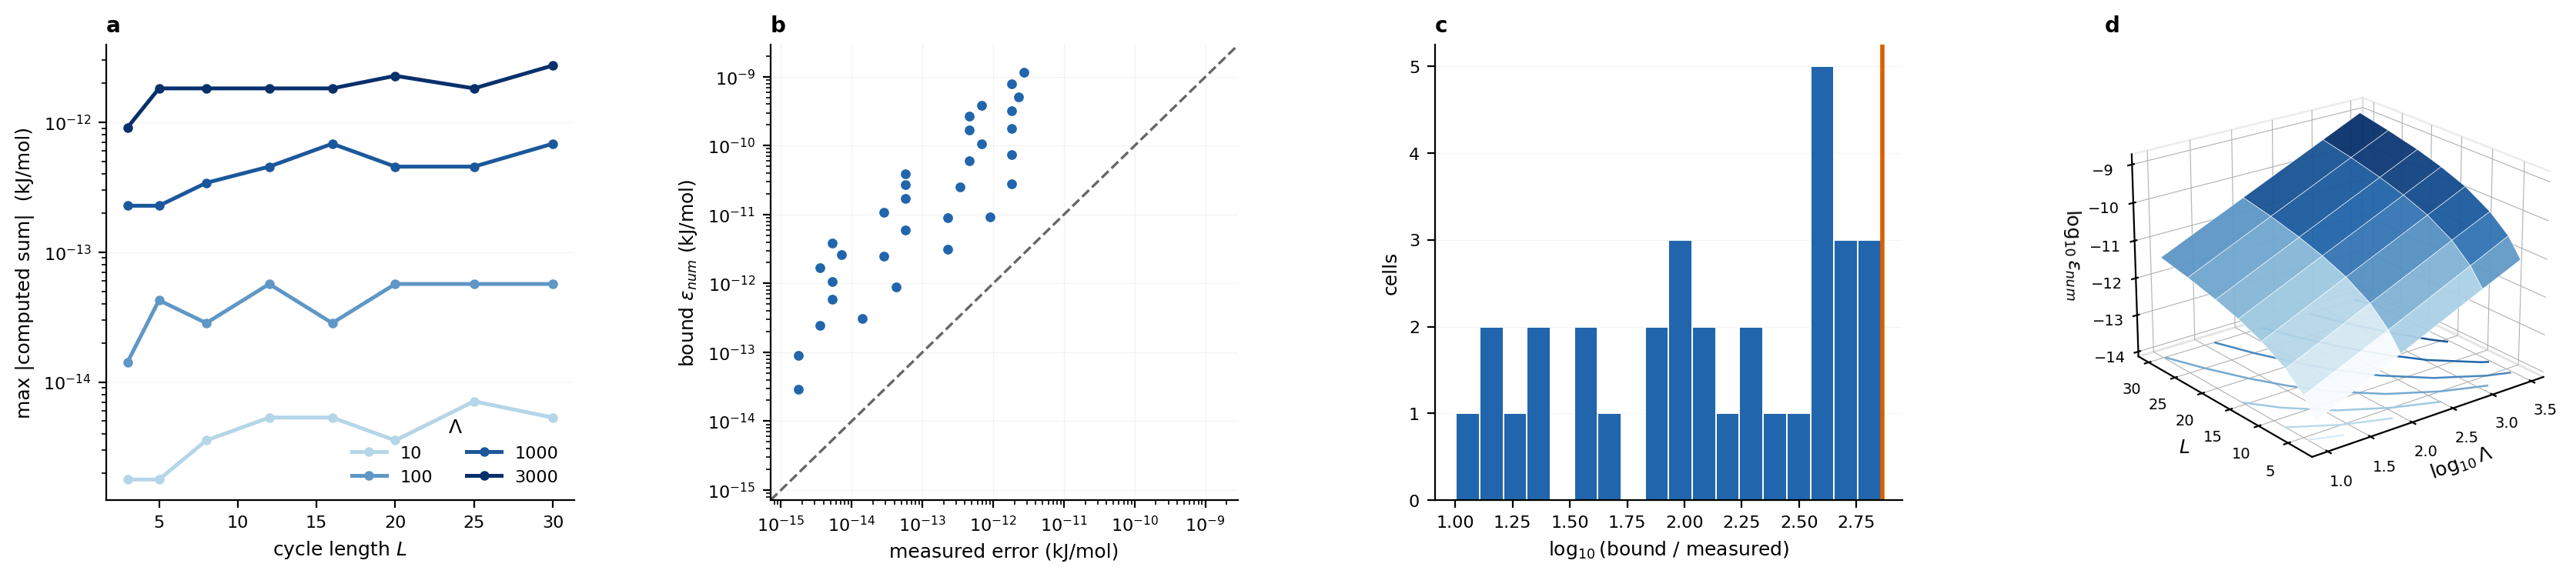
\includegraphics[width=\textwidth]{figures/panel1_numerical_floor.png}
    \caption{\textbf{Rounding error of a computed cycle sum.}
    All quantities are measured on thermodynamically consistent
    circuits, whose cycle sum is identically zero (Lemma 2.8),
    so that the computed value equals the accumulated rounding error.
    IEEE-754 binary64, $\mach = 2^{-53}$.
    (\textbf{A})~Maximum computed $|\widehat{\hol}_\ell|$ over $60$
    random ring circuits per grid cell, against cycle length
    $L\in\{3,5,8,12,16,20,25,30\}$, one curve per potential range
    $\Lambda\in\{10,10^2,10^3,3\times10^3\}$ kJ/mol. The error increases
    with both parameters over three orders of magnitude, from
    $1.78\times10^{-15}$ to $2.73\times10^{-12}$, and its maximum remains
    six orders of magnitude below the conventional threshold $10^{-6}$
    (Remark 3.1).
    (\textbf{B})~Bound $\epsnum(\ell)=\gamma_{2L}\cdot 2L\Lambda_\ell$
    against measured error for all $32$ cells; the dashed diagonal marks
    equality. All points lie above it, with no violation in $1920$
    trials.
    (\textbf{C})~Overestimation factor of the bound: histogram over the
    $32$ cells of the mean bound divided by the maximum measured error
    ($10.1$ to $722$); the orange line marks the median over individual
    trials, $729$. The bound exceeds the observed error by one to three
    orders of magnitude, increasingly with $L$, because it grows as
    $L^{2}$ while random rounding errors accumulate more slowly
    \citep{higham2002}.
    (\textbf{D})~$\log_{10}\epsnum$ as a surface over
    $(\log_{10}\Lambda, L)$, ranging from $2.93\times10^{-14}$ to
    $1.17\times10^{-9}$ kJ/mol. The bound increases in both arguments,
    so it must be computed for each cycle.}
    \label{fig:tol_panel1}
\end{figure}

\subsubsection{Error bound for a computed cycle sum}

\par\noindent\textbf{Theorem 2.12 (Rounding-error bound for a cycle sum).}\label{thm:noise-scale} 
Let $\ell$ be a cycle of length $L=\abs{\ell}$ through species with
potentials bounded by $\Lambda_\ell = \max_{i\in\ell}\abs{\mu_i}$, and
let $\widehat{\hol}_\ell$ denote the value of (4)
computed in the arithmetic of Assumption 2.11 by forming the $L$
differences and summing them in order. Then, although
$\hol_\ell = 0$ exactly,
\begin{equation}
  \bigl\lvert\widehat{\hol}_\ell\bigr\rvert
  \;\le\; \gamma_{2L}\,\cdot\,2L\Lambda_\ell
  \;=\; \frac{2L\mach}{1-2L\mach}\,\cdot\,2L\Lambda_\ell
  \;=\; O\!\left(L^{2}\mach\Lambda_\ell\right).
  \label{eq:noise-bound}
\end{equation}
If the differences are accumulated with compensated (Kahan) summation,
which carries a correction term for the rounding error of each
addition, the bound reduces to $O(L\mach\Lambda_\ell)$.
\par

\noindent\emph{Proof.} See Supplementary Material, Section~S4.

\par\noindent\textbf{Corollary 2.13 (Dependence of the bound on length and potential range).}\label{cor:no-constant} 
Let $\ell_1,\ell_2$ be cycles with $L_1\Lambda_1 \ne L_2\Lambda_2$. Then
the bounds of (7) differ by the factor
$(L_1\Lambda_1)/(L_2\Lambda_2)$, up to the ratio of the $\gamma$ terms,
and no constant $\eps$ lies above the first and below the second
whenever this ratio exceeds the dynamic range required of the test.
\par

\noindent\emph{Proof.} See Supplementary Material, Section~S5.

\par\noindent\textbf{Remark 2.14 (Potential magnitude and potential spread).}\label{rem:lambda} 
The bound is stated in terms of $\Lambda_\ell=\max\abs{\mu_i}$ because
every difference then satisfies $\abs{\Delta\mu_e}\le 2\Lambda_\ell$.
The actual rounding error is governed by a different quantity. A
floating-point subtraction is rounded relative to its result, and by
Sterbenz's lemma it is exact when the two operands lie within a factor
of two of each other \citep{goldberg1991,higham2002}. The error is
therefore determined by the spread $\max\mu-\min\mu$ on the cycle rather
than by the magnitude of the potentials. Standard chemical potentials in
metabolic reconstructions are negative numbers of magnitude
$10^{2}$--$10^{3}$ kJ/mol \citep{alberty1998,noor2013}, whose spread on
a cycle is often much smaller, and the bound in $\max\abs{\mu}$ then
overestimates the error by the ratio of the two. A common shift of all
potentials changes neither a cycle sum nor its rounding error but does
change $\Lambda_\ell$; Section 2.2.3 uses this to reduce the bound.
\par

\subsubsection{Reducing the bound by centring the potentials}
\label{sec:gauge}

\par\noindent\textbf{Proposition 2.15 (Invariance under a common potential shift).}\label{prop:gauge} 
For any $c\in\R$, replacing $\mu$ by $\mu + c\mathbf{1}$ leaves every
cycle sum unchanged but changes the bound (7)
through $\Lambda_\ell$. In the terminology of physics, the choice of
$c$ is a gauge choice. The value minimising the bound on cycle $\ell$ is
$c^{\ast} = -\tfrac{1}{2}(\max_{i\in\ell}\mu_i + \min_{i\in\ell}\mu_i)$,
which gives $\Lambda_\ell = \tfrac{1}{2}(\max_{i\in\ell}\mu_i -
\min_{i\in\ell}\mu_i)$, half the spread.
\par

\noindent\emph{Proof.} See Supplementary Material, Section~S6.

\par\noindent\textbf{Remark 2.16 (Effect of centring on the bound and on the error).}\label{rem:gauge-gain} 
For a cycle through species with potentials $-1750\pm 30$ kJ/mol,
centring reduces $\Lambda_\ell$ from $1780$ to $30$ and the bound by a
factor of approximately $60$. The rounding error itself is unchanged.
Every potential on such a cycle lies within a factor of two of every
other, so by Sterbenz's lemma every difference and every partial sum is
exact, and the computed cycle sum is exactly zero with or without
centring. Centring requires one pass over the cycle and changes no
reported quantity; it reduces the overestimation of the bound, not the
error of the computation. It is applied throughout, and both components
of the tolerance are reported in the protocol (Supplementary
Section~S16).
\par

% =====================================================================
\subsection{Uncertainty threshold}
\label{sec:data-floor}
% =====================================================================

\subsubsection{Propagation of uncertainty to a cycle sum}

The rounding-error bound of Section 2.2 applies to exact
reaction data. Measured and estimated data are not exact. Standard
Gibbs energies estimated by group- or component-contribution methods
carry reported uncertainties of several kJ/mol
\citep{alberty1998,noor2013,flamholz2012}, and concentrations carry
measurement uncertainty. Only part of this uncertainty affects a cycle
sum.

\par\noindent\textbf{Lemma 2.17 (Cancellation of species-level errors).}\label{lem:species-cancel} 
Let the reaction data be differences of estimated species potentials,
$d=B^{\top}\hat\mu$ with $\hat\mu_i=\mu_i+\eta_i$ for arbitrary errors
$\eta_i$. Then $\hol_\ell(d)=0$ for every cycle $\ell$ and every $\eta$.
\par

\noindent\emph{Proof.} See Supplementary Material, Section~S7.

Concentrations enter each reaction datum through the terms $RT\ln c_i$
of its two endpoints, so concentration uncertainty does not reach a
cycle sum. The same applies to the uncertainty of standard Gibbs
energies of formation when reaction Gibbs energies are computed from
them \citep{noor2013}. Reaction data constructed in this way are
consistent by construction, and a cycle-sum test applied to them detects
only errors of bookkeeping. Thermodynamic inconsistency arises from
reaction data that are not derived from a single potential vector:
reaction Gibbs energies or equilibrium constants measured or annotated
reaction by reaction, or ratios of forward and reverse rate constants,
which the Haldane relation links to the standard reaction Gibbs energy
\citep{schuster1989}. A model of uncertainty attached to species
potentials therefore predicts no variation of the cycle sum, as the
simulations of Section 3.2 confirm.

\par\noindent\textbf{Definition 2.18 (Uncertainty of a reaction datum).}\label{def:sigma} 
Each reaction datum $d_e$ carries an uncertainty $\sigma_e>0$, the
reported standard error of the part of $d_e$ that is estimated
independently for that reaction.
\par

\par\noindent\textbf{Theorem 2.19 (Uncertainty threshold for a cycle sum).}\label{thm:data-floor} 
Let $d_e=\bar d_e+\eta_e$ with $\bar d$ consistent and the errors
$\eta_e$ independent with standard deviations $\sigma_e$. Then the cycle
sum $\hol_\ell(d)$ has mean zero and standard deviation
\begin{equation}
  s_\ell \;=\; \Bigl(\textstyle\sum_{e\in E} z_\ell(e)^{2}\,
  \sigma_e^{2}\Bigr)^{1/2},
  \label{eq:data-sd}
\end{equation}
which for a simple cycle is $s_\ell=(\sum_{e\in\ell}\sigma_e^{2})^{1/2}$.
With
\begin{equation}
  \epsdata(\ell) \;=\; z_{1-\alpha/2}\; s_\ell,
  \label{eq:data-floor}
\end{equation}
where $z_{1-\alpha/2}$ is the standard normal quantile, a consistent
network satisfies $\abs{\hol_\ell} \le \epsdata(\ell)$ with probability
$1-\alpha$ when the $\eta_e$ are normally distributed.
\par

\noindent\emph{Proof.} See Supplementary Material, Section~S7.

\par\noindent\textbf{Remark 2.20 (Reaction data without reported uncertainty).}\label{rem:no-sigma} 
Many reconstructions report no uncertainty for individual reactions
\citep{brunk2018,orth2010}, and the uncertainty threshold cannot then be
computed. No default value is substituted, since an assumed $\sigma$
would turn a question the data cannot answer into an apparently definite
answer. The protocol of Section 2.8 instead reports $\epsdata$ as
undefined and assigns the intermediate class of Theorem 2.27 to
every cycle whose sum exceeds $\epsnum$.
\par

% =====================================================================
\subsection{Cycle-specific tolerance}
\label{sec:tolerance}
% =====================================================================

\subsubsection{Definition and error guarantees}

\par\noindent\textbf{Definition 2.21 (Cycle-specific tolerance).}\label{def:epsstar} 
For a cycle $\ell$, the \emph{cycle-specific tolerance} is
\begin{equation}
  \epsstar(\ell) \;=\; \epsnum(\ell)+\epsdata(\ell),
  \label{eq:epsstar}
\end{equation}
with $\epsnum(\ell)$ the bound (7) of
Theorem 2.12, computed after centring (Proposition 2.15), and
$\epsdata(\ell)$ the threshold (9) of
Theorem 2.19. If no uncertainties are supplied, $\epsdata$ is
undefined and Remark 2.20 applies.
\par

\par\noindent\textbf{Remark 2.22 (Sum of the two components).}\label{rem:sum-not-max} 
A computed cycle sum contains rounding error and data error together,
so the tolerance must cover both. If the maximum of the two components
were used in place of their sum, neither Theorem 2.23
nor Theorem 2.24 would hold in the presence of data error. In
all settings reported here $\epsnum/\epsdata<10^{-9}$, so the two
definitions agree to the precision reported.
\par

\par\noindent\textbf{Theorem 2.23 (False-positive bound).}\label{thm:no-false-positive} 
Let the network be consistent, $\delta(d)=0$ in the sense of
Definition 2.9, and let the potentials be exact. Then for every
cycle $\ell$ the computed sum satisfies
$\abs{\widehat{\hol}_\ell} \le \epsstar(\ell)$ deterministically. If
the reaction data carry independent errors as in
Theorem 2.19, the event $\abs{\widehat{\hol}_\ell} >
\epsstar(\ell)$ has probability at most $\alpha$.
\par

\noindent\emph{Proof.} See Supplementary Material, Section~S8.

\par\noindent\textbf{Theorem 2.24 (Detection guarantee).}\label{thm:detection} 
Suppose a defect is present with cycle sum $\abs{\hol_\ell} = D$ on a
cycle $\ell$, and $D > 2\epsstar(\ell)$. If the reaction data are
otherwise exact, the computed value satisfies
$\abs{\widehat{\hol}_\ell} > \epsstar(\ell)$ and the test flags $\ell$.
If they carry independent errors as in Theorem 2.19, the test
flags $\ell$ with probability at least $1-\alpha$.
\par

\noindent\emph{Proof.} See Supplementary Material, Section~S9.

\par\noindent\textbf{Remark 2.25 (Decision threshold and detection limit).}\label{rem:factor2} 
Theorems 2.23 and 2.24 correspond to the two limits
of detection theory in analytical chemistry \citep{currie1968}:
$\epsstar$ is the decision threshold (critical level), above which a
result is reported as a detection, and $2\epsstar$ is the detection
limit, the smallest true defect detected with probability at least
$1-\alpha$. For a defect between $\epsstar$ and $2\epsstar$ detection is
not guaranteed. The width of this interval is determined by the
precision of the arithmetic and of the data, and it can be reduced only
by improving either. A fixed tolerance does not remove the interval; it
assigns every value within it to one of the two outcomes.
\par

\subsubsection{Three-valued classification}

\par\noindent\textbf{Definition 2.26 (Verdict).}\label{def:verdict} 
For a cycle $\ell$ with computed sum $\widehat{\hol}_\ell$, the
\emph{verdict} is
\begin{equation}
  \mathrm{verdict}(\ell) =
  \begin{cases}
    \textsf{CONSISTENT}   & \abs{\widehat{\hol}_\ell} \le
                            \epsnum(\ell),\\[2pt]
    \textsf{UNDECIDABLE}  & \epsnum(\ell) < \abs{\widehat{\hol}_\ell}
                            \le \epsstar(\ell),\\[2pt]
    \textsf{INCONSISTENT} & \abs{\widehat{\hol}_\ell} > \epsstar(\ell).
  \end{cases}
  \label{eq:verdict}
\end{equation}
\textsf{UNDECIDABLE} denotes that the data supplied do not determine the
classification; it is not used in the sense of computability theory.
\par

\par\noindent\textbf{Theorem 2.27 (Properties of the three-valued classification).}\label{thm:trichotomy} 
\leavevmode
\begin{enumerate}[label=(\roman*),leftmargin=2em,itemsep=2pt]
\item The three cases of (11) are exhaustive and mutually
exclusive.
\item The class \textsf{UNDECIDABLE} is non-empty whenever
$\epsdata(\ell) > 0$, that is, for every cycle whose reaction data carry
independently estimated uncertainty. In realistic cases $\epsdata$
exceeds $\epsnum$ by many orders of magnitude.
\item Any fixed rule that reduces the three classes to two either
classifies as consistent some cycles whose sum exceeds the rounding-error
bound, or classifies as inconsistent some cycles whose sum lies within
the data uncertainty. Neither classification is supported by the data.
\end{enumerate}
\par

\noindent\emph{Proof.} See Supplementary Material, Section~S10.

\begin{figure}[!htbp]
    \centering
    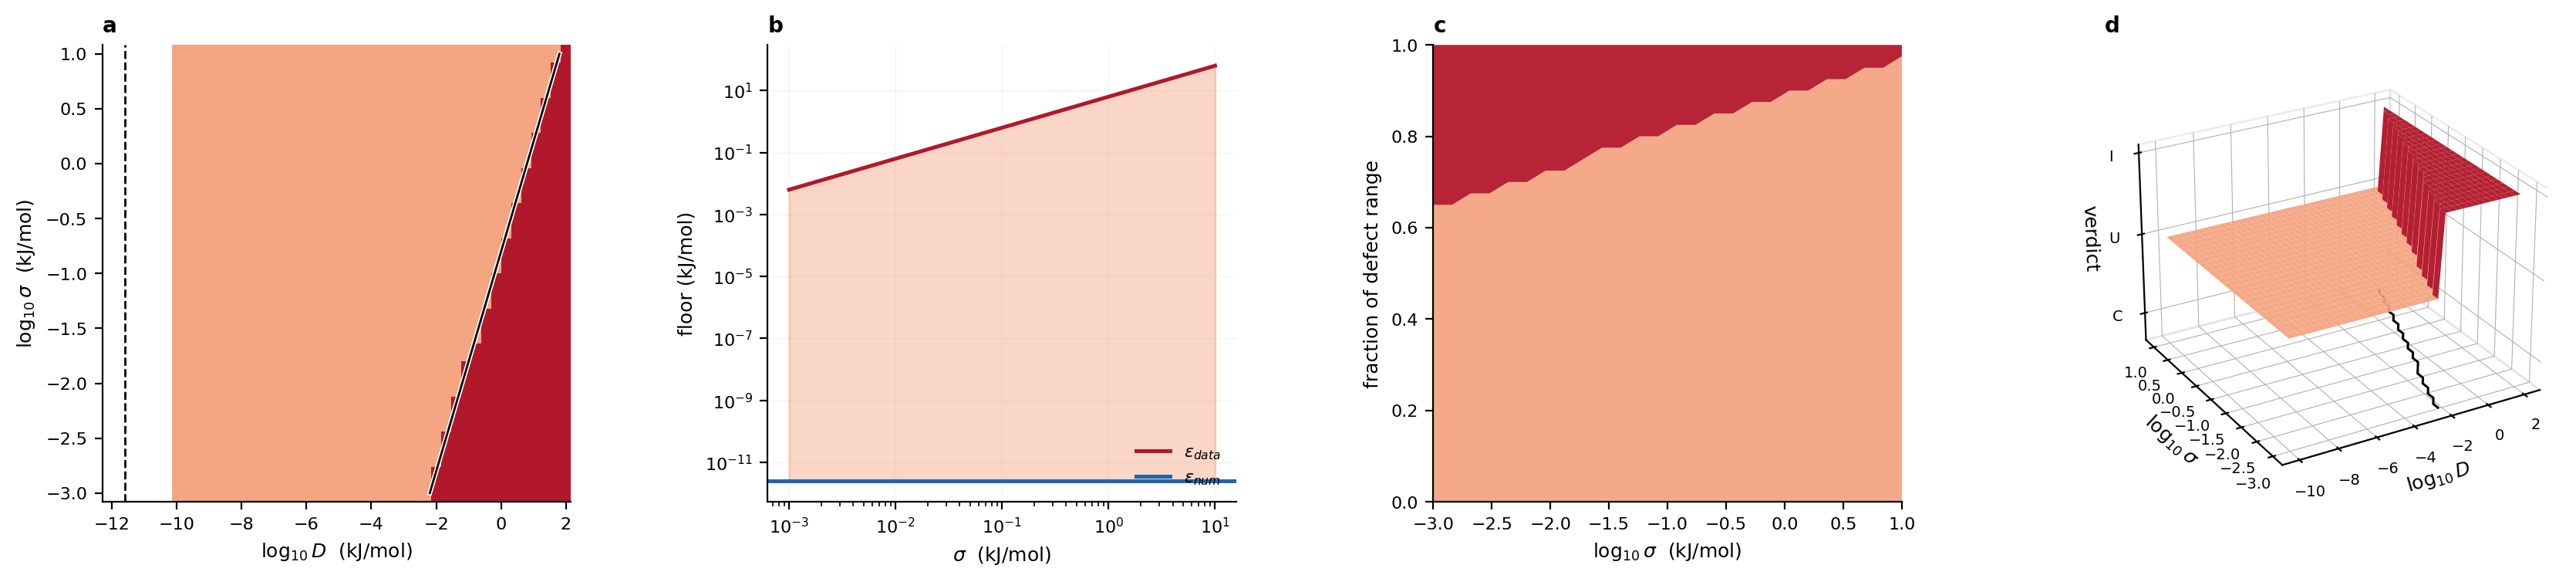
\includegraphics[width=\textwidth]{figures/panel3_trichotomy.png}
    \caption{\textbf{Three-valued classification as a function of data
    uncertainty and defect magnitude.}
    A six-edge cycle at $\Lambda=200$ kJ/mol on a $26\times40$ grid of
    per-reaction uncertainty $\sigma\in[10^{-3},10]$ against injected
    defect $D\in[10^{-10},10^{2}]$ kJ/mol ($1040$ points), with
    noise-free reaction data, so that each verdict is determined by $D$
    and the two components of the tolerance.
    (\textbf{A})~Verdict map: blue \textsf{CONSISTENT}, orange
    \textsf{UNDECIDABLE}, red \textsf{INCONSISTENT}. The solid curve is
    $\epsdata(\sigma)$, which equals $\epsstar$ to within $10^{-9}$; the
    dashed vertical line is $\epsnum=2.48\times10^{-12}$ kJ/mol. The
    orange region between them covers $80.9\%$ of the grid.
    (\textbf{B})~The two components against $\sigma$. The rounding-error
    bound is constant at $2.48\times10^{-12}$; the uncertainty threshold
    increases from $6.31\times10^{-3}$ to $63.1$ kJ/mol. At the midpoint
    of the range they differ by $11.5$ orders of magnitude
    (Theorem 2.27(ii)).
    (\textbf{C})~Proportion of each verdict against $\sigma$. The
    \textsf{INCONSISTENT} proportion decreases from $0.350$ to $0.025$ as
    data uncertainty increases; at $\sigma=10$ the test returns
    \textsf{UNDECIDABLE} on $97.5\%$ of the defect range, all of which a
    two-valued rule would have classified.
    (\textbf{D})~The verdict as a surface over
    $(\log_{10}D, \log_{10}\sigma)$. No \textsf{CONSISTENT} region
    appears because the sweep begins at $D=10^{-10}$, forty times
    $\epsnum$ (Section 3.2).}
    \label{fig:tol_panel3}
\end{figure}

\par\noindent\textbf{Remark 2.28 (Information carried by the intermediate class).}\label{rem:undecidable} 
The class \textsf{UNDECIDABLE} conveys information that a two-valued
test discards: the cycle sum is too large to be rounding error and too
small to be resolved by data of the given quality. It also specifies
what would resolve it, namely a reduction of the uncertainties
$\sigma_e$ on the reactions of $\ell$ to below
$\abs{\widehat{\hol}_\ell}/\epsdata(\ell)$ of their present values.
\par

% =====================================================================
\subsection{Dependence on the choice of cycle basis}
\label{sec:basis}
% =====================================================================

\subsubsection{Invariance of the network-level classification}

\par\noindent\textbf{Theorem 2.29 (Basis independence of the verdict).}\label{thm:basis-verdict} 
Let $\mathcal{B}_1,\mathcal{B}_2$ be cycle bases of $G$ and let $d$ be
reaction data. Then $z^{\top}d = 0$ for all $z\in\mathcal{B}_1$ if and
only if $z^{\top}d=0$ for all $z\in\mathcal{B}_2$. Consequently the
classification of the network as consistent or inconsistent does not
depend on the basis.
\par

\noindent\emph{Proof.} See Supplementary Material, Section~S11.

\subsubsection{Basis dependence of the flagged cycles}

\par\noindent\textbf{Proposition 2.30 (Basis dependence of the flagged set).}\label{prop:basis-localisation} 
There exist a graph $G$, reaction data $d$ with a single defective edge
$e^{\ast}$, and cycle bases $\mathcal{B}_1,\mathcal{B}_2$ of $G$ such
that exactly one element of $\mathcal{B}_1$ has a nonzero cycle sum,
while three elements of $\mathcal{B}_2$ do.
\par

\noindent\emph{Proof.} See Supplementary Material, Section~S12.

\par\noindent\textbf{Remark 2.31 (Consequence for the reporting of localisation).}\label{rem:loc-consequence} 
By Proposition 2.30, the statement that a defect is
localised to cycle $\ell$ depends both on the network and on the basis
computed by the implementation. A protocol that reports localisation
must therefore either fix a canonical basis and state it, or report a
basis-independent quantity. The second approach is adopted here.
\par

\subsubsection{Witness set}

\par\noindent\textbf{Definition 2.32 (Flagged set and witness set).}\label{def:witness} 
Fix a cycle basis $\mathcal{B}$ and let
$F(\mathcal{B}) = \{\ell\in\mathcal{B} :
\mathrm{verdict}(\ell)=\textsf{INCONSISTENT}\}$ be the flagged set. The
\emph{witness set} is
\begin{equation}
  W(\mathcal{B}) \;=\; \bigcap_{\ell\in F(\mathcal{B})} E(\ell),
  \label{eq:witness}
\end{equation}
the set of edges that lie on every flagged cycle, with
$W = \emptyset$ when $F=\emptyset$.
\par

\par\noindent\textbf{Theorem 2.33 (Containment of the defective edge in the witness set).}\label{thm:witness-contains} 
Suppose that exactly one edge $e^{\ast}$ is defective, with defect $D >
2\max_\ell \epsstar(\ell)$, and that the remaining reaction data are
exact. Then for every cycle basis $\mathcal{B}$, $e^{\ast}\in
W(\mathcal{B})$, and $F(\mathcal{B})$ is the set of basis cycles with a
nonzero net traversal of $e^{\ast}$; for simple cycles, these are the
cycles containing $e^{\ast}$. If the reaction data carry independent
errors as in Theorem 2.19, the same holds with probability at
least $1-\nu\alpha$.
\par

\noindent\emph{Proof.} See Supplementary Material, Section~S13.

\par\noindent\textbf{Corollary 2.34 (Basis-independent localisation).}\label{cor:localise-witness} 
The basis-independent content of a positive result is that the defect
lies in $W(\mathcal{B})$. The cardinality $\abs{W}$ measures the
resolution of the localisation: $\abs{W}=1$ identifies a single
reaction, and a large $\abs{W}$ indicates that the flagged cycles share
many edges, which the test cannot distinguish.
\par

\par\noindent\textbf{Remark 2.35 (Effect of a minimum cycle basis).}\label{rem:mcb} 
Theorem 2.33 holds for every basis, but short cycles
share fewer edges, so a minimum-weight cycle basis (a basis of least
total length; \citealp{horton1987,kavitha2009}) generally yields a
smaller $W$ and hence a finer localisation. Such a basis is used in the
protocol of Section 2.8, and $\abs{W}$ is reported as a primary
outcome in place of a single cycle.
\par

\begin{figure}[!htbp]
    \centering
    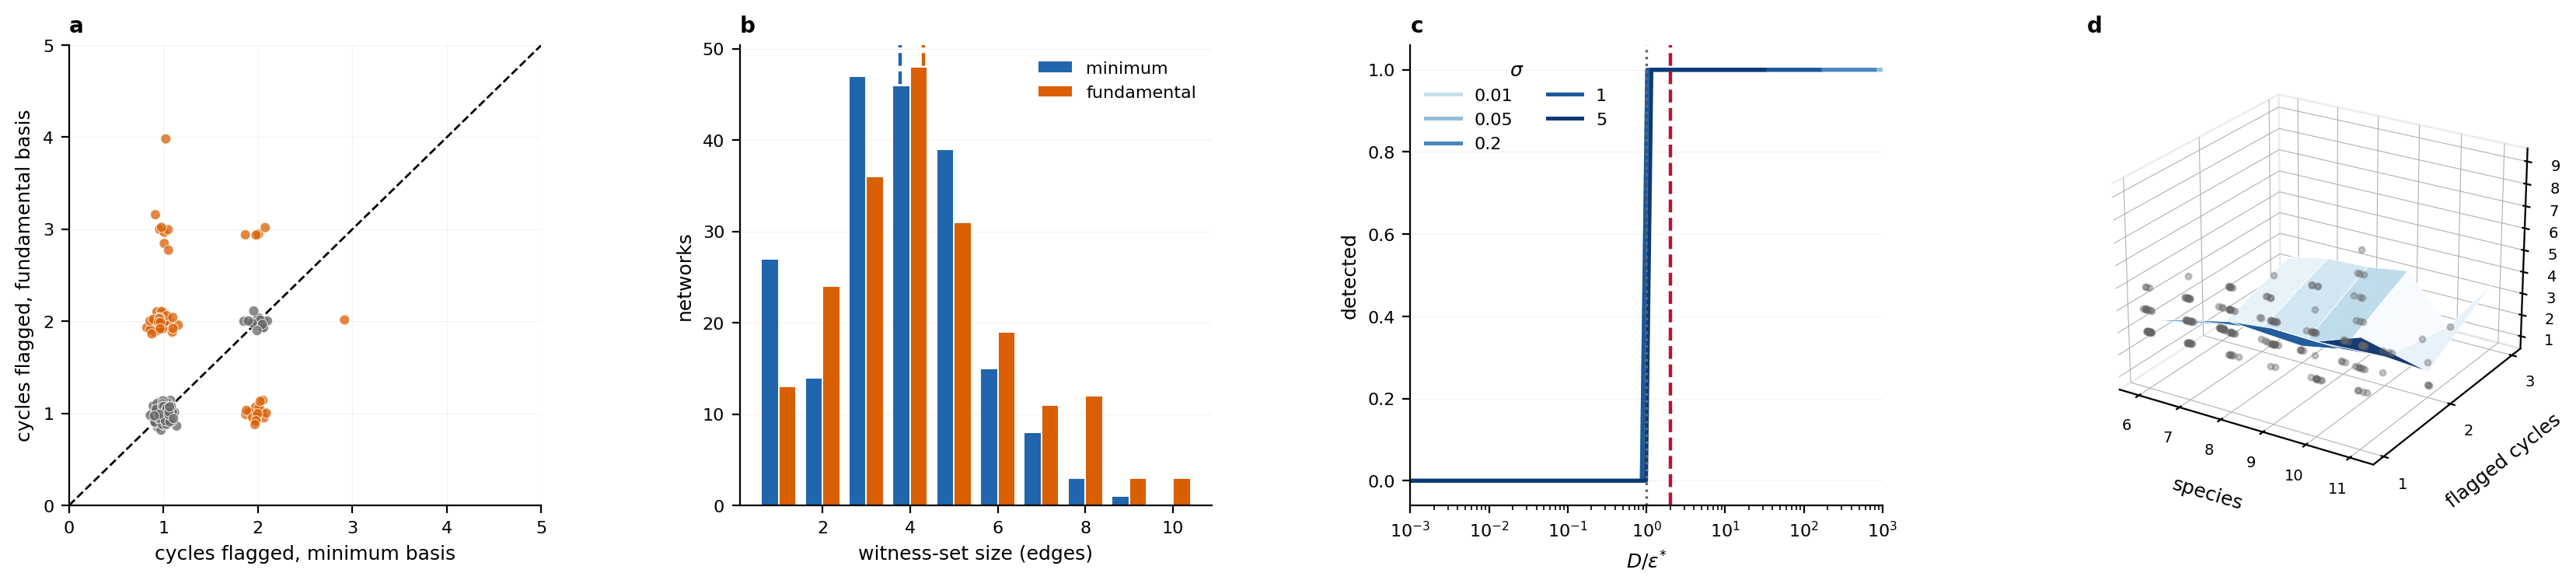
\includegraphics[width=\textwidth]{figures/panel4_basis_detection.png}
    \caption{\textbf{Basis dependence of localisation and invariance of
    the witness set.}
    Panels (A), (B) and (D) use $200$ random networks of $6$ to $11$
    species with $2$ to $4$ chords (edges outside a spanning tree), each
    with one edge defect of $50$ kJ/mol and $\sigma=0.05$ kJ/mol; panel
    (C) is an independent detection sweep.
    (\textbf{A})~Number of cycles flagged under a minimum-weight basis
    against a fundamental basis (the basis formed by one spanning tree
    and its chords), with jitter to separate coincident integer points.
    Orange points indicate disagreement: $69/200$ trials ($34.5\%$). The
    network-level verdict agreed in $200/200$ trials
    (Theorem 2.29).
    (\textbf{B})~Witness-set cardinality
    $|W|=|\bigcap_{\ell\in F}E(\ell)|$ for each basis, with means shown
    dashed. The minimum-weight basis gives a finer localisation ($3.77$
    against $4.30$ edges; Remark 2.35), by less than half an edge.
    Both bases contained the defective edge in $200/200$ trials
    (Theorem 2.33).
    (\textbf{C})~Detection rate against $D/\epsstar$ for five data
    qualities $\sigma\in\{0.01,0.05,0.2,1,5\}$ kJ/mol, $220$ points
    each, on noise-free reaction data. The dotted vertical line marks
    $\epsstar$ and the dashed line the detection limit $2\epsstar$ of
    Theorem 2.24. Without noise the verdict depends on $D$ only
    through $D/\epsstar$, so the curves coincide by construction and
    change at $\epsstar$ ($0.51$ to $0.58$ of $2\epsstar$, the spread
    reflecting the spacing of the $D$ grid); the guarantee under noise
    is tested in V6 (Section 3.2).
    (\textbf{D})~Mean witness-set size against network size and number
    of flagged cycles. Localisation becomes coarser as more cycles are
    flagged (Pearson $r=-0.72$): because the witness set is an
    intersection, fine localisation requires short cycles with little
    overlap.}
    \label{fig:tol_panel4}
\end{figure}

% =====================================================================
\subsection{Validity of the reference network}
\label{sec:validity}
% =====================================================================

The cycle-consistency test presupposes that the network as supplied
admits a potential function. If the thermodynamic annotations of the
reconstruction are themselves inconsistent, cycles are flagged for
reasons unrelated to any disease state, and the test provides no
diagnostic information.

\par\noindent\textbf{Definition 2.36 (Validity check).}\label{def:validity} 
A network with reaction data $d$ \emph{passes the validity check} if no
cycle $\ell$ of the chosen basis receives the verdict
\textsf{INCONSISTENT} on the reference (nominally healthy) parameter
set, with each $\epsdata(\ell)$ computed at level $\alpha/\nu$, so that
a consistent reference network passes with probability at least
$1-\alpha$.
\par

The check requires the absence of \textsf{INCONSISTENT} verdicts rather
than \textsf{CONSISTENT} verdicts throughout, because a consistent
network with uncertain reaction data is expected to return
\textsf{UNDECIDABLE}; \textsf{CONSISTENT} is attainable only for data
that are exactly potential differences.

\par\noindent\textbf{Criterion 2.37 (Invalid versus negative).}\label{crit:invalid} 
An experiment in which the reference network fails
Definition 2.36 is \textbf{invalid}, not negative. It shows that the
thermodynamic annotations of the reconstruction are not consistent to
the precision they report, and it supports no conclusion about the
diagnostic. An experiment in which the reference network passes and a
perturbed network is not flagged is \textbf{negative}: it shows that
the test does not detect that perturbation at that data quality.
\par

\par\noindent\textbf{Remark 2.38 (Pre-registration of the criterion).}\label{rem:preregister} 
If Criterion 2.37 is not stated in advance, a failed reference
check can be attributed to the data when the diagnostic succeeds and to
the method when it fails. Fixing the interpretation before the data are
examined removes this freedom of interpretation
\citep{simmons2011,sandve2013}.
\par

% =====================================================================
\subsection{Experimental data}
\label{sec:data}

\paragraph{Cycles in a stoichiometric network.} Most reactions have
several substrates or products, so a realistic network is described by
a stoichiometric matrix $S$ (species by reactions) rather than by a
graph; Section 2.1 treats the special case $S=B$. A cycle is an
integer vector $z\in\ker S$, and its sum is $\hol_z=z^{\top}d$. All
results above carry over with integer coefficients $z_\ell(e)$ in place
of $\pm1$: if $d=S^{\top}\mu$ then $\hol_z=(Sz)^{\top}\mu=0$, which gives
Lemmas 2.8 and 2.17, and the proof of
Theorem 2.19 is unchanged. For reaction data supplied directly,
the rounding-error bound is
$\epsnum(z)=\gamma_{\abs{z}}\sum_e\abs{z_e d_e}$, with $\abs{z}$ the
number of reactions in the cycle (Supplementary Section~S17). The kernel
of $S$ is spanned by an integer basis computed in exact rational
arithmetic.

\paragraph{Equilibrium constants from TECRDB.} The Thermodynamics of
Enzyme-Catalyzed Reactions Database (TECRDB; \citealp{goldberg2004})
records apparent equilibrium constants $K'$ measured for individual
reactions, each with the pH, ionic strength, temperature and pMg (the
negative decadic logarithm of the free magnesium concentration) of the
measurement. Measurements graded A to C at $293$ to $313$ K were
admitted. Each reaction was balanced with water and protons, and
$-RT\ln K'$ was converted by the reverse Legendre transform to the
standard reaction Gibbs energy in the chemical reference state at the
conditions of measurement, following the procedure by which the
component-contribution method prepares its training data
\citep{noor2013,beber2022}. The resulting values
$d_e=\Delta_rG^{\circ}_e$ are independent measurements and not
differences of formation energies, which would cancel on every cycle
and make the test vacuous. Each study contributes one value per
reaction, and $\sigma_e=\sigma/\sqrt{n_e}$ for a reaction measured in
$n_e$ studies, with $\sigma$ the pooled between-study standard
deviation.

\paragraph{Human erythrocyte reaction network.} For $38$ enzymes
covering the published erythrocyte models \citep{mulquiney1999}, every
catalytic activity annotated in UniProtKB/Swiss-Prot
\citep{uniprot2025} was retrieved together with the stoichiometry of its
Rhea reaction \citep{bansal2022}. Compounds were identified by molecular
connectivity, so that anomers (stereoisomers of a sugar differing only
at the anomeric carbon) are merged, and ion pumps were reduced to their
net chemical reaction. Reactions with generic participants were
excluded. All data were retrieved on 21 October 2026; the snapshot, its
checksums and the analysis are provided in the repository.

\subsection{Implementation and protocol}
\label{sec:language}
\label{sec:protocol}

\paragraph{Typed implementation.} A correctly computed $\epsstar$ is of
no use if the comparison is subsequently written against a literal
constant, as in \verb|if abs(H) > 1e-6|. The test is therefore expressed
in a small typed language in which the only operation producing a
\cf{Verdict} requires a \cf{Tolerance} as an argument. Consequently, no
well-typed program yields a verdict without its tolerance, and the
comparison of a cycle sum with a numeric literal is a type error
(Supplementary Section~S15). The type system guarantees that the
tolerance is computed and recorded; it does not guarantee that the
inputs are correct, and a program supplied with an incorrect $\sigma_e$
is well-typed and gives an incorrect result.

\paragraph{Experimental protocol and pre-registered criteria.}
Supplementary Section~S16 specifies the protocol in executable detail:
the network \citep{brunk2018}; the thermodynamic
\citep{noor2013,flamholz2012} and physiological
\citep{rapoport1975,mulquiney1999} data; and a perturbation of the
forward rate constant of pyruvate kinase alone, which violates the
Haldane relation and introduces a defect of
$RT\ln(1/0.15)\approx4.9$ kJ/mol on that edge. Three controls are
included, each designed so that it can fail on correctly formed input,
and the criteria for success and failure are fixed in advance. One
control scales the forward and reverse rate constants by the same
factor, corresponding to the loss of activity observed in clinical
pyruvate kinase deficiency \citep{zanella2005}; this perturbation
preserves every cycle sum and must not be flagged. The criteria
distinguish a \emph{negative} experiment from an \emph{invalid} one: by
Criterion 2.37, a reference network that fails its consistency
check supports no conclusion about the diagnostic. Applied to the
erythrocyte network of Section 2.7, the protocol terminates at its
third step, which requires the perturbed edge to lie on a cycle
(Section 3.3).

% =====================================================================
\section{Results and Discussion}
\label{sec:results}

Section 3.1 quantifies the performance of a fixed
tolerance. Section 3.2 reports the computational validation
of the numbered results, Section 3.3 applies the test to
experimental data, and Section 3.4 discusses the limitations of
the approach.

\subsection{Performance of a fixed tolerance}
\label{sec:fixed-tolerance-fails}
% =====================================================================

All numbers in this section are produced by the validation suite
described in Section 3.2, and the construction is specified in
full so that it can be reproduced exactly.

\subsubsection{Magnitude of rounding error in double precision}

\begin{table}[t]
\centering\small
\caption{Measured rounding error of cycle sums of consistent circuits,
whose exact value is zero, so that the computed value equals the error.
Binary64. Each entry is the maximum over $60$ random circuits with
potentials drawn uniformly from $[-\Lambda,\Lambda]$, so that $\Lambda$
also determines their spread. The error increases with both $L$ and
$\Lambda$, as Theorem 2.12 predicts, over three orders of
magnitude; its largest value is $2.7\times10^{-12}$.}
\label{tab:v1}
\begin{tabular}{@{}lrrrr@{}}
\toprule
& \multicolumn{4}{c}{$\Lambda$ (kJ/mol)}\\
\cmidrule(l){2-5}
$L$ & $10$ & $100$ & $1000$ & $3000$\\
\midrule
$3$  & $3.6\times10^{-15}$ & $2.8\times10^{-14}$ & $2.3\times10^{-13}$ & $9.1\times10^{-13}$\\
$8$  & $3.6\times10^{-15}$ & $2.8\times10^{-14}$ & $3.4\times10^{-13}$ & $1.8\times10^{-12}$\\
$16$ & $5.3\times10^{-15}$ & $5.7\times10^{-14}$ & $6.8\times10^{-13}$ & $1.8\times10^{-12}$\\
$30$ & $5.3\times10^{-15}$ & $5.7\times10^{-14}$ & $6.8\times10^{-13}$ & $2.7\times10^{-12}$\\
\bottomrule
\end{tabular}
\end{table}

Table 1 reports the measured rounding error. In $1920$ trials
covering $L\in[3,30]$ and $\Lambda\in[10,3000]$ kJ/mol, the bound of
Theorem 2.12 was never violated. The bound overestimates the
error: its median ratio to the observed error is $729$, and the ratio
increases with $L$, from about $180$ at $L=3$ to $2200$ at $L=30$ for
$\Lambda=1000$ kJ/mol, because the bound grows as $L^{2}$ while random
rounding errors accumulate more slowly \citep{higham2002}.

The largest rounding error in Table 1, $2.7\times10^{-12}$, lies
six orders of magnitude below $10^{-6}$. In binary64 a fixed threshold
of $10^{-6}$ therefore cannot flag any consistent circuit of the grid as
a result of rounding, and the measured false-positive rate was $0.000$
in all four strata of Figure 4A ($1600$ trials).

\par\noindent\textbf{Remark 3.1 (Position of the conventional threshold).}\label{rem:prediction-failed} 
Corollary 2.13 holds: the rounding error varies with
$L\Lambda$ over three orders of magnitude in Table 1. The
corollary does not imply that the conventional threshold lies within
this range, and in binary64 it lies above all of it. The case for a
computed tolerance in double precision therefore rests on the
uncertainty of the data and on detection sensitivity, not on rounding.
\par

\begin{figure}[!htbp]
    \centering
    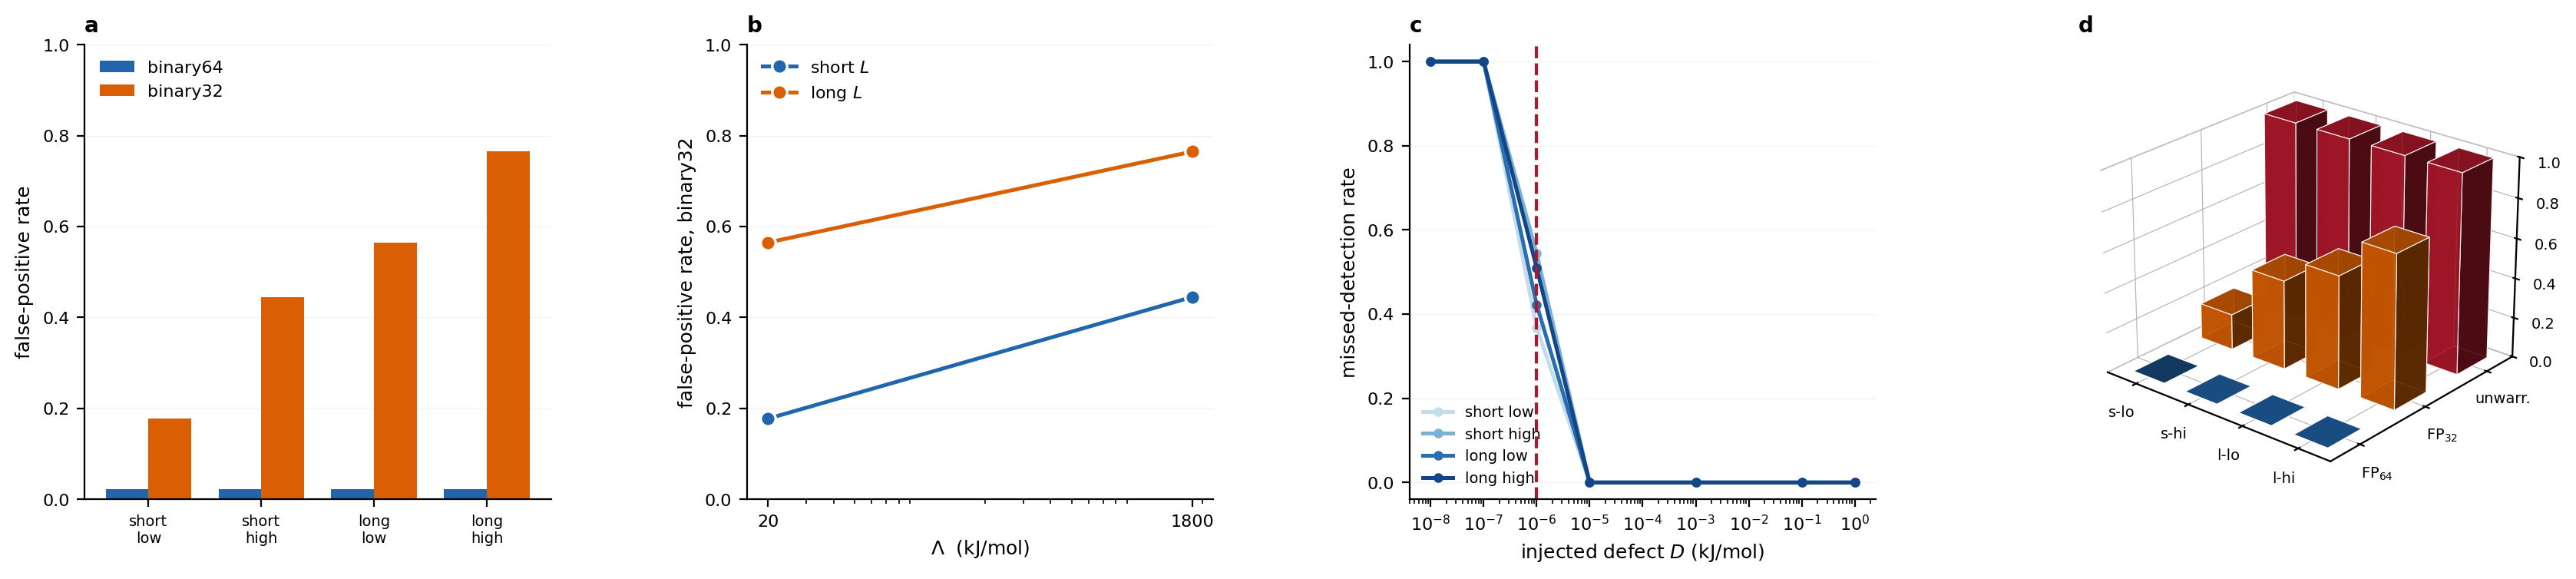
\includegraphics[width=\textwidth]{figures/panel2_fixed_tolerance.png}
    \caption{\textbf{Performance of a fixed tolerance $\eps=10^{-6}$.}
    Four strata of $400$ trials, combining short ($L\in[3,5]$) or long
    ($L\in[15,22]$) cycles with a low ($\Lambda=20$ kJ/mol) or high
    ($\Lambda=1800$ kJ/mol) potential range.
    (\textbf{A})~False-positive rate on consistent circuits: $0.000$ in
    every stratum in binary64 (bars of zero height;
    Remark 3.1); the same null experiment in binary32
    gives $0.177$, $0.445$, $0.565$ and $0.765$.
    (\textbf{B})~The binary32 rate by length class against $\Lambda$.
    The length has the larger effect, so the rate is not monotone in
    $L\Lambda$.
    (\textbf{C})~Missed-detection rate against injected defect
    $D\in[10^{-8},1]$ kJ/mol, with $\eps$ dashed. Every defect below the
    threshold is missed in every stratum, and none is missed at
    $D=10^{-5}$. The threshold acts as a detection limit rather than as
    a filter for rounding error.
    (\textbf{D})~The three error types per stratum. With $\sigma=1$
    kJ/mol and a defect of $0.5$ kJ/mol, which lies within that
    uncertainty, the fixed test returns \textsf{INCONSISTENT} on every
    cycle for which the cycle-specific test returns
    \textsf{UNDECIDABLE}. This, rather than the false-positive rate, is
    the principal deficiency of the fixed tolerance.}
    \label{fig:tol_panel2}
\end{figure}

\subsubsection{Missed detections and unsupported positive results}

Figure 4 distinguishes the errors that a fixed tolerance
makes from those it does not make.

\paragraph{Detection limit imposed by the threshold.} At $D=10^{-7}$ the
missed-detection rate is $1.000$ in every stratum
(Figure 4C), although these cycle sums are computed almost
exactly. The misses result from a threshold chosen by convention rather
than from the smallest defect of interest. A numerical solver setting
thus imposes a detection limit of $10^{-6}$ kJ/mol that has no
biochemical justification.

\paragraph{Classification of defects within the data uncertainty.} With
a per-reaction uncertainty of $\sigma=1$ kJ/mol and an injected defect of
$0.5$ kJ/mol, the fixed test returns \textsf{INCONSISTENT} on $100\%$ of
cycles, since $0.5 \gg 10^{-6}$, whereas the cycle-specific test returns
\textsf{UNDECIDABLE} (Figure 4D). A two-valued test cannot
express that a cycle sum lies far above the rounding error and far
below the resolution of the data, and is forced to report a result that
the data do not support. Section 3.3 shows the same behaviour on
measured data.

\paragraph{False positives in single precision.} When the null
experiment is repeated in binary32, where $\mach\approx6\times10^{-8}$
and the rounding-error bound approaches $10^{-6}$, the false-positive
rate increases from $0.177$ to $0.765$ with both $L$ and $\Lambda$, and
is not monotone in their product (Figure 4B), since $L$
enters Theorem 2.12 quadratically and $\Lambda$ linearly.
$\epsnum$ must therefore be computed for each cycle from both
quantities.

% =====================================================================
\subsection{Computational validation}
\label{sec:validation}
% =====================================================================

Each numbered result of Section 2 was checked computationally.
Table 2 summarises the experiments.

\subsubsection{Design of the validation suite}

For an identity, a computational check verifies the implementation; for
a bound, it measures the overestimation factor (V1). Experiments V3 and
V5 use noise-free reaction data, for which each verdict is a
deterministic function of the defect and the two components of the
tolerance; they therefore map the structure of the classification
rather than test a probabilistic claim. The probabilistic statements are
tested by simulating noise in V6. Defects are always introduced on an
edge (Remark 3.2), and V1, V4 and V6 each contain a
negative control, a check that an effect does not occur on correctly
formed input.

\begin{table}[t]
\centering\small
\caption{Validation suite. Every experiment is seeded, and the JSON
record is the source of every number reported in this article.}
\label{tab:validation}
\begin{tabular}{@{}llll@{}}
\toprule
& Result tested & Trials & Outcome\\
\midrule
V1 & Theorem 2.12 & $1920$ & $0$ violations; median ratio $729$\\
V2 & Section 3.1 & $1600$ & no false positives in binary64\\
V3 & Theorem 2.27 & $1040$ & noise-free map;
\textsf{UNDECIDABLE} $=80.9\%$\\
V4 & Theorem 2.29 and Proposition 2.30 & $200$ &
verdicts agree; flagged sets differ in $34.5\%$\\
V5 & Theorem 2.24 & $1100$ & noise-free; $0$ violations\\
V6 & Lemma 2.17, Theorems 2.19, 2.23 and 2.24 & $24{,}000$ &
FP $0.009$ at $\alpha=0.01$; detection $\ge0.993$\\
\bottomrule
\end{tabular}
\end{table}

\par\noindent\textbf{Remark 3.2 (Introduction of defects on reactions).}\label{rem:edge-not-node} 
A defect cannot be introduced by shifting a species potential $\mu_i$:
the shifted reaction data remain potential differences, so by
Lemma 2.8 every cycle sum remains zero and no defect is
detected. An inconsistency can be introduced only on an edge
(Definition 2.9). Because a perturbation of a species potential
produces a null result indistinguishable from a genuine negative, V6
contains a negative control verifying that such a perturbation is not
detected.
\par

\subsubsection{Extent of the undecidable region (V3)}

Theorem 2.27(ii) states only that the class
\textsf{UNDECIDABLE} is non-empty. In a sweep of
$\sigma\in[10^{-3},10]$ kJ/mol against $D\in[10^{-10},10^{2}]$ kJ/mol
on a six-membered cycle at $\Lambda=200$ kJ/mol ($1040$ grid points;
Figure 2), the verdict was \textsf{UNDECIDABLE} on $80.9\%$
of the grid and \textsf{INCONSISTENT} on $19.1\%$. These proportions
depend on the limits of the sweep; the separation between the two
components of the tolerance, $11.5$ orders of magnitude near the middle
of the $\sigma$ range, does not. The \textsf{CONSISTENT} proportion of
$0.000$ results from the lower limit of the sweep, which is forty times
the rounding-error bound.

\subsubsection{Basis dependence of localisation (V4)}

On $200$ random networks of $6$ to $11$ species with $2$ to $4$ chords,
each carrying a single edge defect of $50$ kJ/mol
(Figure 3A,B), the network-level verdict agreed between a
minimum-weight and a fundamental basis in all trials ($0/200$
disagreements), as Theorem 2.29 requires. The two bases
flagged different numbers of cycles in $69/200$ trials ($34.5\%$), so a
report localising the defect to a single cycle would have depended on
the basis in about one trial in three
(Proposition 2.30). The witness set contained the
defective edge in $200/200$ trials under both bases
(Theorem 2.33). The minimum-weight basis gave a finer
localisation, as Remark 2.35 predicts, by less than half an edge
($3.77$ against $4.30$ edges). A witness set of about four edges
identifies a region of the network rather than a single reaction, and
is reported as such.

\subsubsection{Detection with and without data noise (V5, V6)}

Theorem 2.24 guarantees detection when $D>2\epsstar$. On
noise-free reaction data (V5), with $D$ swept over $220$ points at each
of five data qualities, $\sigma\in\{0.01,0.05,0.2,1,5\}$ kJ/mol, the
guarantee was violated in none of $1100$ evaluations
(Figure 3C). Without noise a defect is detected as soon as
it exceeds $\epsstar$, that is, at $0.51$ to $0.58$ of $2\epsstar$, the
spread reflecting the grid spacing. The factor of two is required only
for the guarantee under noise (Remark 2.25).

V6 introduces noise on ring cycles of length $L\in\{4,8,16\}$ with
$\sigma\in\{0.1,1\}$ kJ/mol, $4000$ trials per configuration and
$\alpha=0.01$. Independent normal errors on the species potentials left
the verdict \textsf{CONSISTENT} in all $24{,}000$ trials, as
Lemma 2.17 requires, whereas a model of uncertainty
attached to the species would predict a cycle-sum standard deviation of
$\sqrt{L}\,\sigma$. Independent normal errors on the reaction data gave
false-positive rates of $0.008$ to $0.011$ (mean $0.009$), against the
nominal $0.01$ of Theorem 2.23, and a defect of
$2\epsstar$ was detected with frequency $0.9935$ to $0.996$, against the
guaranteed $0.99$ of Theorem 2.24. A defect of $\epsstar$, below
the detection limit, was detected with frequency $0.49$ to $0.51$.

% =====================================================================
\subsection{Application to measured data}
\label{sec:measured}
% =====================================================================

\begin{figure}[!htbp]
    \centering
    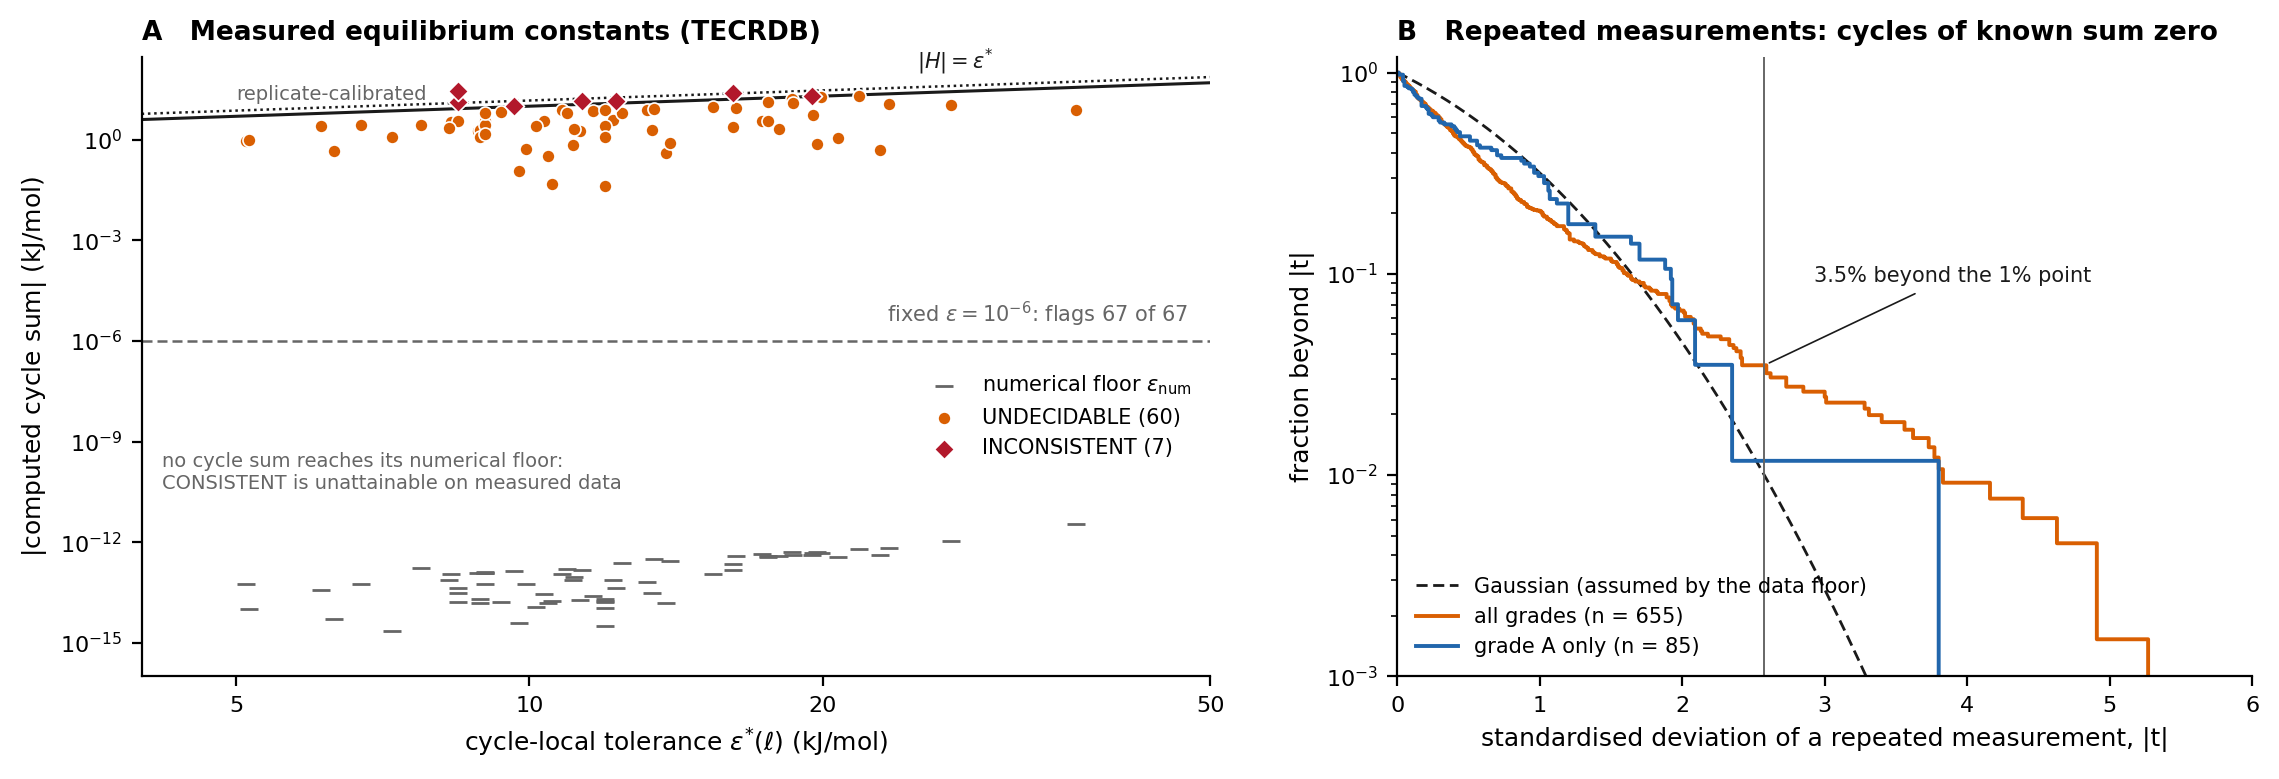
\includegraphics[width=\textwidth]{figures/panel5_measured_data.png}
    \caption{\textbf{The test applied to measured equilibrium
    constants.}
    (\textbf{A})~Each of the $67$ cycles spanning the cycle space of the
    $418$ reactions measured in TECRDB: computed sum against
    cycle-specific tolerance (Gaussian uncertainty threshold), with the
    rounding-error bound (grey dash) fourteen orders of magnitude lower.
    Every sum exceeds the fixed $\eps=10^{-6}$; $7$ exceed $\epsstar$
    (solid line) and $3$ exceed the tolerance calibrated on replicate
    measurements (dotted line).
    (\textbf{B})~Leave-one-out deviations between studies of the same
    reaction, which form cycles of known sum zero. Across all quality
    grades the tail is heavier than the Gaussian distribution assumed by
    the uncertainty threshold; grade-A data follow the Gaussian
    distribution.}
    \label{fig:tol_panel5}
\end{figure}

\paragraph{Fixed tolerances on TECRDB cycles.} The admitted TECRDB data
comprise $3{,}276$ measurements from $908$ studies of $418$ reactions,
of which $165$ were measured in more than one study (between-study
standard deviation $\sigma=2.68$ kJ/mol). The cycle space has dimension
$67$, with cycles of $3$ to $25$ reactions (Figure 5A).
All cycle sums lie between $0.042$ and $27.8$ kJ/mol. A fixed
tolerance of $10^{-6}$ or $10^{-3}$ therefore classifies all $67$ cycles
as inconsistent, and tolerances of $1$, $5$ or $10$ kJ/mol classify
$54$, $27$ or $14$ as inconsistent: the outcome is determined by the
choice of $\eps$. The rounding-error bounds lie between
$2.3\times10^{-15}$ and $3.4\times10^{-12}$ kJ/mol and the uncertainty
thresholds between $5.1$ and $36.4$ kJ/mol, a median separation of
$14.1$ orders of magnitude, so that \textsf{CONSISTENT} cannot be
attained on measured data. The cycle-specific tolerance returns
\textsf{UNDECIDABLE} for $60$ cycles and \textsf{INCONSISTENT} for $7$.

\paragraph{Calibration of the uncertainty threshold.}
Theorem 2.19 uses a Gaussian quantile. Two studies of the same
reaction form a cycle whose true sum is zero, so the $655$ leave-one-out
deviations of a study from the remaining studies test this assumption
on the data themselves (Figure 5B). They exceed the
Gaussian $1\%$ point in $3.5\%$ of cases, and their $99$th percentile is
$3.81$ standard deviations instead of $2.58$. With this empirical
quantile the test flags $3$ cycles; with the distribution-free quantile
$\alpha^{-1/2}=10$ given by Chebyshev's inequality (Supplementary
Section~S7) it flags none. The heavy tail originates in the lower
quality grades: restricted to grade A, the replicates follow the
Gaussian distribution ($1.2\%$ beyond its $1\%$ point, $\sigma=1.49$
kJ/mol), and $2$ of $13$ cycles are flagged under either quantile. V6
establishes the false-positive rate under Gaussian noise only; for
measured data the quantile must first be calibrated on replicate
measurements.

\paragraph{Localisation with multiple defects.} Over $200$ fundamental
bases of the same cycle space, at least one cycle was flagged in every
basis, as Theorem 2.29 requires, but the number of flagged
cycles ranged from $2$ to $40$ and the witness set of
Definition 2.32 was empty. The data therefore contain several
independent inconsistencies, a case outside the scope of
Theorem 2.33 (Section 3.4). In this case the
quantity that localises is the frequency with which a reaction lies on
a flagged cycle. The single measurement of
pyrophosphate--fructose-6-phosphate 1-phosphotransferase lies on a
flagged cycle in $94\%$ of bases; its cycle with inorganic
pyrophosphatase and fructose-bisphosphatase sums to $-27.8$ kJ/mol,
$8.5$ standard deviations from zero (Supplementary Section~S17).

\paragraph{Human erythrocyte network.} The $38$ enzymes carry $118$
annotated reactions, of which $70$ are chemically distinct and fully
specified, over $101$ species. The cycle space has dimension $7$, and
only $19$ of the $70$ reactions lie on a cycle. A reaction that lies on
no cycle does not enter any cycle sum, so no cycle-consistency test can
detect a defect on it, regardless of the data. Pyruvate kinase is such
a reaction, since no erythrocyte enzyme converts pyruvate back to
phosphoenolpyruvate. The same holds for every glycolytic step except
phosphoglycerate kinase and phosphoglycerate mutase, which lie on the
only cycle through glycolysis: the Rapoport--Luebering shunt, the bypass
of phosphoglycerate kinase through 2,3-bisphosphoglycerate, closed by
ATP hydrolysis. TECRDB contains no measurement for bisphosphoglycerate
mutase or bisphosphoglycerate phosphatase, the enzymes of the shunt; the
other six cycles pass through nucleotide kinases, and none of the seven
cycles has a measured equilibrium constant for every reaction. The
protocol accordingly terminates at its third step, as pre-registered.
With the present data the test cannot be applied to the erythrocyte;
measurements for the two enzymes of the shunt would make one cycle
testable.

% =====================================================================
\subsection{Limitations}
\label{sec:limits}
% =====================================================================

\paragraph{Conditions of measurement.} A correction applied to species
potentials, such as an activity coefficient, cancels around every cycle
(Lemma 2.17). Differences between the conditions under
which individual reaction data were obtained do not cancel.
Section 2.7 removes the dependence on pH, ionic strength and
magnesium by the reverse Legendre transform, but not the temperature
dependence of $\Delta_rG^{\circ}$, which is limited by admitting only
measurements at $293$ to $313$ K. Where TECRDB reports no ionic strength
or magnesium concentration, $I=0.25$ M and the absence of magnesium are
assumed. Both residual effects are systematic, contribute to the
between-study spread, and are absorbed by the calibration described in
Section 3.3.

\paragraph{Steady-state assumption.} The circuit representation of
Proposition 2.4 holds at steady state. A network under transient
conditions has no time-invariant potential function, and cycle sums
computed from instantaneous concentrations are not the quantity analysed
here.

\paragraph{Correlated uncertainties.} Theorem 2.19 assumes
that the errors of the reaction data are independent. Two measurements
from the same laboratory are not independent, and each study therefore
contributes one value per reaction (Section 2.7). Reaction Gibbs
energies estimated from shared group contributions are also correlated
\citep{noor2013}, but the part of the correlation that arises from
common formation energies cancels around every cycle
(Lemma 2.17).

\paragraph{Defects undetectable by cycle sums.} The test detects
reaction data that are not potential differences, on reactions that lie
on a cycle, and no other perturbation. A loss of enzyme activity that
scales the forward and reverse rate constants by the same factor, which
is the usual molecular consequence of an enzyme deficiency, preserves
the Haldane relation and therefore every cycle sum; so does any
perturbation of concentrations alone (Lemma 2.17). A
reaction that lies on no cycle, such as pyruvate kinase in the
erythrocyte, cannot be tested at all.

\paragraph{Network assembly.} The erythrocyte network merges anomers and
reduces ion pumps to their net chemical reaction, neglecting the
membrane potential. Both simplifications can only add cycles, so they
do not affect the finding that pyruvate kinase lies on no cycle.

\paragraph{Multiple defects.} Theorem 2.33 assumes a
single defective edge. Measured data contain several, and the witness
set is then empty (Section 3.3). The appropriate generalisation
is the family of minimal edge sets that intersect every flagged cycle,
which is a hitting-set problem and is not developed here; the frequency
with which an edge lies on a flagged cycle serves as a heuristic
substitute.

\paragraph{Conservatism of the rounding-error bound.}
Equation (7) is a standard worst-case bound, quadratic in $L$,
and exceeds the observed error by one to three orders of magnitude
(V1). Since $\epsdata$ exceeds it by fourteen orders of magnitude on
measured data, this conservatism changes no verdict reported here.

% =====================================================================
\section{Conclusion}
\label{sec:conclusion}
% =====================================================================

The cycle sum of a thermodynamically consistent metabolic network is
zero as an algebraic identity. A diagnostic based on it must therefore
distinguish rounding error and data uncertainty from a genuine defect,
and a fixed tolerance treated as a solver setting does not make this
distinction. In double precision the conventional $\eps=10^{-6}$
produces no false positives from rounding; its deficiency is that it
classifies as inconsistent cycle sums that the data cannot resolve, and
on measured equilibrium constants all $67$ cycle sums exceed it. The
cycle-specific tolerance replaces it by the sum of a rounding-error
bound and an uncertainty threshold derived from reaction-level
uncertainty alone. The separation of fourteen orders of magnitude
between the two components makes the classification three-valued: on
measured data, $60$ cycles are undecidable and $7$ inconsistent.

The analysis of experimental data required two refinements of the
method. The Gaussian quantile of the uncertainty threshold is too small
for the database as a whole, and replicate measurements, which form
cycles of known sum zero, provide the calibration. The witness set
assumes a single defect, whereas the measured data contain several. The
experimental data also delimit the application. In the human
erythrocyte, pyruvate kinase lies on no cycle and no cycle is fully
measured, so no erythrocyte defect can be examined by a
cycle-consistency test with the present data; measurements for the two
enzymes of the Rapoport--Luebering shunt would make one cycle testable.
Whether disease states produce reaction data that are not potential
differences remains an open question.

% =====================================================================
\section*{Reproducibility}
% =====================================================================

The validation suite of Section 3.2 is in
\texttt{validation/run\_validation.py}, is seeded
(\texttt{seed}~$=20260819$), and writes every quantity reported in this
article to \texttt{validation/results.json}; the tables of
Sections 3.1 and 3.2 are read from that file.
Figures~1--4 and the graphical abstract are generated from it (the
latter also from \texttt{results\_real.json}) by \texttt{validation/make\_panels.py} and
\texttt{validation/make\_graphical\_abstract.py}, so no plotted value is
computed independently of a reported one. The analysis of
Section 3.3 is in \texttt{validation/realdata/}:
\texttt{fetch\_sources.py} saves the TECRDB, UniProt and Rhea data with
their SHA-256 checksums, \texttt{run\_realdata.py} writes
\texttt{results\_real.json}, and Figure~5 is drawn from it. Its first
stage needs the eQuilibrator compound cache (Zenodo,
doi:10.5281/zenodo.4128543); the second runs from the derived tables it
writes. No step requires proprietary software, wet-lab work, or
computation beyond a single workstation.

% =====================================================================
\section*{Funding Support}
% =====================================================================

%% TODO(author): replace with the actual funder and grant number, or
%% keep the "no specific grant" wording if that is accurate.
This research received no specific grant from any funding agency in the
public, commercial, or not-for-profit sectors.

% =====================================================================
\section*{Ethical Statement}
% =====================================================================

This study does not contain any studies with human or animal subjects
performed by the author. All data used are computationally generated or
drawn from public databases of previously published measurements.

% =====================================================================
\section*{Conflicts of Interest}
% =====================================================================

The author declares no conflict of interest.

% =====================================================================
\section*{Data Availability Statement}
% =====================================================================

%% TODO(author): insert the public repository URL and DOI before
%% submission. The journal expects a location and access conditions.
The data supporting the findings of this study are openly available.
The seeded validation suite (\texttt{run\_validation.py}), the complete
record of every quantity reported here (\texttt{results.json}), and the
figure-generation scripts are deposited in a public repository,
together with the snapshot of experimental data analysed in
Section 3.3, retrieved on 21 October 2026 from TECRDB
\citep{goldberg2004}, UniProtKB \citep{uniprot2025} and Rhea
\citep{bansal2022}, all publicly available, and the tables derived from
it.

% =====================================================================
\section*{Author Contribution Statement}
% =====================================================================

\textbf{Kundai Farai Sachikonye:} Conceptualization, Methodology,
Formal analysis, Software, Validation, Investigation, Visualization,
Writing -- original draft, Writing -- review \& editing. The author
has read and agreed to the published version of the manuscript.

% =====================================================================
\bibliographystyle{apacite}
\bibliography{references}

\end{document}
